\subsection{Bài 1: Delay}
Hàm \texttt{delay(xn, xorigin, k)} thực hiện phép trễ tín hiệu:
\[
y(n) = x(n - k) \quad (k > 0)
\]
\begin{itemize}
    \item \textbf{Đầu vào:} Vector tín hiệu \texttt{xn}, vị trí gốc thời gian \texttt{xorigin}, số mẫu trễ \texttt{k}.
    \item \textbf{Đầu ra:} Vector tín hiệu sau trễ \texttt{yn}, vị trí gốc thời gian mới \texttt{yorigin}.
\end{itemize}

\noindent\textbf{Thực thi:}\\
Cho tín hiệu $x(n) = \{1, -2, \underset{\uparrow}{3}, 6\}$, $xorigin = 3$. Thực hiện trễ $k = 1$ mẫu:\\
Gọi hàm: \texttt{[yn, yorigin] = delay([1, -2, 3, 6], 3, 1)}
\begin{itemize}
    \item Kết quả: \texttt{yn = [1, -2, 3, 6]}, \texttt{yorigin = 2}
    \item Giải thích: Khi làm trễ 1 mẫu, toàn bộ dạng sóng dịch sang phải 1 đơn vị trên trục thời gian. Vị trí gốc thời gian $n = 0$ chuyển từ index 3 sang $3 - 1 = 2$.
\end{itemize}

\begin{figure}[H]
    \centering
    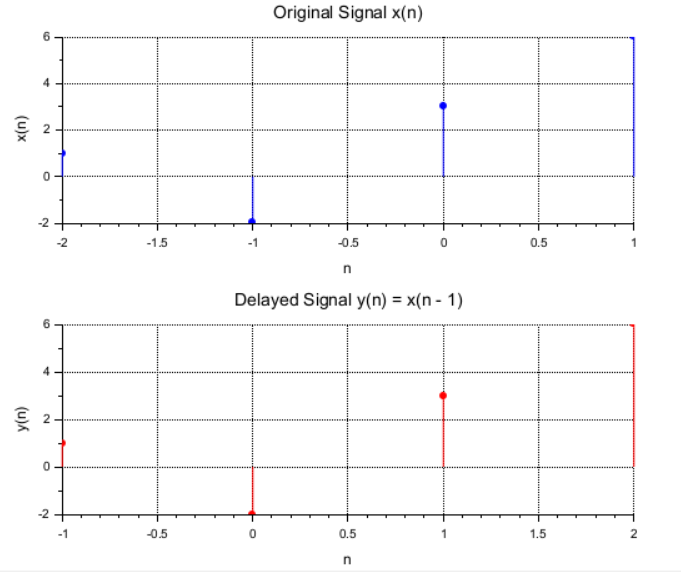
\includegraphics[width=0.65\textwidth]{img/ex1.png}
    \caption{Đồ thị tín hiệu gốc $x(n)$ và tín hiệu trễ $y(n) = x(n - 1)$}
\end{figure}

\noindent$\rightarrow$ \textbf{Nhận xét:} Tín hiệu sau khi trễ giữ nguyên biên độ của các mẫu, dạng sóng bị dịch sang phải 1 mẫu theo đúng lý thuyết.
